\documentclass[twoside,11pt]{article}

% Any additional packages needed should be included after jmlr2e.
% Note that jmlr2e.sty includes epsfig, amssymb, natbib and graphicx,
% and defines many common macros, such as 'proof' and 'example'.
%
% It also sets the bibliographystyle to plainnat; for more information on
% natbib citation styles, see the natbib documentation, a copy of which
% is archived at http://www.jmlr.org/format/natbib.pdf

\usepackage{jmlr2e}

\usepackage[acronym]{glossaries} %Used for the acronyms
\usepackage{mathtools} %tools for mathematical writing
\usepackage{caption}
\usepackage{subfig}
\usepackage{float}
\usepackage{color}
\usepackage{adjustbox}
\usepackage{comment}
\usepackage{hyperref} % For hyperlinks in the PDF
\usepackage{algorithm}% http://ctan.org/pkg/algorithms
\usepackage{algpseudocode}% http://ctan.org/pkg/algorithmicx
\usepackage[acronym]{glossaries} %Used for the acronyms
\usepackage[titletoc]{appendix}

% Definitions of handy macros can go here

\newcommand{\dataset}{{\cal D}}
\newcommand{\fracpartial}[2]{\frac{\partial #1}{\partial  #2}}

% Heading arguments are {volume}{year}{pages}{date submitted}{date published}{paper id}{author-full-names}

\jmlrheading{18}{2018}{1-48}{07/18}{10/00}{dlaredo00a}{Laredo, Chen, Sun and Sch\"{u}tze}

% Short headings should be running head and authors last names

\ShortHeadings{A Neural Network-Evolutionary Computation Framework for Remaining Useful Life Estimation}{Laredo, Chen,  Sun and Sch\"{u}tze}
\firstpageno{1}

\begin{document}

\title{A Neural Network-Evolutionary Computation Framework for Remaining Useful Life Estimation}

%Term definitions
\newacronym{rul}{RUL}{Remaining Useful Life}
\newacronym{mlp}{MLP}{Multi-layer Perceptron}
\newacronym{cmaps}{C-MAPSS}{Commercial Modular Aero Propulsion System Simulator}
\newacronym{ann}{ANN}{Arificial Neural Networks}
\newacronym{cbm}{CBM}{Condition Based Maintenance}
\newacronym{pmh}{PMH}{Prognostics and Health Management}
\newacronym{ml}{ML}{Machine Learning}



%Remove after the paper is complete.
\newacronym{moo}{MOO}{Multi-objective Optimization}
\newacronym{mop}{MOP}{Multi-objective Optimization Problem}
\newacronym{mmop}{MMOP}{Mixed-Integer Multi-objective Optimization Problem}
\newacronym{eds}{EDS}{Enhanced Directed Search}
\newacronym{dzz}{DZZ}{Direct Zig Zag}
\newacronym{nsga2}{NSGA-II}{Non-Sorted Genetic Algorithm II}
\newacronym{sop}{SOP}{Single-objective Optimization Problem}
\newacronym{pc}{PC}{Predictor-Corrector}
\newacronym{moea}{MOEA}{Multi-objective Optimization Evolutionary Algorithm}
\newacronym{ea}{EA}{Evolutionary Algorithm}
\newacronym{ds}{DS}{Directed Search}
\newacronym{kkt}{KKT}{Karush-Kuhn-Tucker}
\newacronym{bop}{BOP}{Bi-objective Optimization Problem}
\newacronym{gd}{GD}{Generational Distance}
\newacronym{igd}{IGD}{Inverted Generational Distance}
\newacronym{gsa}{GSA}{Gradient Subspace Approximation}
\newacronym{ift}{IFT}{Implicit Function Theorem}
\newacronym{fps}{FPS}{First Pareto Solution}
\newacronym{moead}{MOEA-D}{Multi-objective Optimization Evolutionary Algorithm based on Decomposition}
\newacronym{pf}{PF}{Pareto Front}
\newacronym{nbi}{NBI}{Normal Boundary Intersection}
\newacronym{pso}{PSO}{Particle Swarm Optimization}
 %Insert acronym list

%Used to not expand the first acronym
\glsunsetall

\author{\name David Laredo \email dlaredorazo@ucmerced.edu \\
			 \name Zhaoyin Chen \email zchen@ucmerced.edu \\
			 \name Jian-Qiao Sun \email jsun3@ucmerced.edu \\
       \addr Department of Mechanical Engineering\\
       University of California\\
       Merced, Ca 95340-5200, USA
       \AND
       \name Oliver Sch\"{u}tze \email schuetze@cs.cinvestav.mx \\
       \addr Department of Computer Science\\
       CINVESTAV\\
       Mexico City, Av. Instituto Politecnico Nacional 07360-1776, Mexico}

\editor{Kevin Murphy and Bernhard Sch{\"o}lkopf}

\maketitle

\begin{abstract}%   <- trailing '%' for backward compatibility of .sty file
This paper presents a data-driven framework for estimating the remaining useful life (\gls{rul}) of mechanical systems. Two major components make up the framework: a multi-layer perceptron as base regressor and an evolutionary computation algorithm for the tuning of data-related parameters. On the data side, the framework makes use of a strided time window along with a piecewise linear model to estimate the \gls{rul} label for each time window within the training sets. Tuning the data-related parameters using the optimization framework here presented allows for the use of simple regressor models, e.g. neural networks with few hidden layers and few neurons at each layer, which can in turn be deployed in environments with very limited resources such as embedded systems. The proposed method is evaluated on the publicly available \gls{cmaps} dataset. The accuracy of the proposed method is compared against other state-of-the art methods available in the literature and it is shown to perform better while making use of a simpler, compact model.
\end{abstract}

\begin{keywords}
  Artificial Neural Networks, Moving Time Window, \gls{rul} Estimation, Prognostics, Evolutionary Algorithms
\end{keywords}

%----------------------------------------------------------------------------------------
%	ARTICLE CONTENTS
%----------------------------------------------------------------------------------------

\section{Introduction}

Traditionally, maintenance of mechanical systems has been carried out based on scheduling strategies, nevertheless strategies such as breakdown corrective maintenance and scheduled preventive maintenance are often costly and less capable of meeting the increasing demand of efficiency and reliability \cite{gebraeel_2005, zaidan_2013}. Condition Based Maintenance (\gls{cbm}) also known as intelligent Prognostics and Health Management (\gls{pmh}) allows for maintenance based on the current health of the system, thus cutting costs and increasing the reliability of the system \cite{zhao_2017}. To avoid confusion, here we define prognostics as the estimation of remaining useful component life. The Remaining Useful Life (\gls{rul}) of a system can be estimated based on history trajectory data, this approach which we refer here as data-driven can help improve maintenance schedules to avoid engineering failures and save costs \cite{lee_2014}. This paper proposes a Machine Learning (\gls{ml}) approach for \gls{rul} estimation.

The existing \gls{pmh} methods can be grouped into three different categories: model-based approaches \cite{yu_2001} , data-driven approaches \cite{liu_2009, mosallam_2013} and hybrid approaches \cite{pecht_2010, liu_2012}.

Model-based approaches attempt to incorporate physical models of the system into the estimation of the \gls{rul}. If the system degradation is modeled  precisely, model-based approaches usually exhibit better performance than data-driven approaches \cite{qian_2017}, nevertheless this comes at the expense of having extensive a prior knowledge of the underlying system and having a fine-grained model of such system (which usually involve expensive computations). On the other hand data-driven approaches tend to use pattern recognition to detect changes in system states. Data-driven approaches are appropriate when the understanding of first principles of system operation is not comprehensive or when the system is sufficiently complex (i.e. jet engines, car engines, complex machinery) such that developing an accurate model is prohibitively expensive. Common disadvantages for the data-driven approaches are that they usually exhibit wider confidence intervals than model-based approaches and that a fair amount of data is required for training.
\section{NASA C-MAPSS Dataset}
\label{sec:rul_dataset}

The NASA \gls{cmaps} dataset \cite{CMAPS2008} is used to evaluate performance of the proposed method. The \gls{cmaps} dataset contains simulated data produced using a model based simulation program (Commercial Modular Aero-Propulsion System Simulation) developed by NASA. The dataset is further divided into 4 subsets composed of multi-variate temporal data obtained from 21 sensors.

For each of the 4 subsets a training and a test set is provided. The training sets include run-to-failure sensor records of multiple aero-engines collected under different operational conditions and fault modes as described in Table \ref{table:cmapss}.

\begin{table}[!htb]
\centering
\begin{tabular}{l | l l l l}
	\hline
	 & \multicolumn{4}{c}{C-MAPSS}\\  
	 Dataset & FD001 & FD002 & FD003 & FD004\\
  	\hline
  	Train Trajectories & 100 & 260 & 100 & 248\\
  	Test Trajectories & 100 & 259 & 100 & 248\\
  	Operating Conditions & 1 & 6 & 1 & 6\\
  	Fault Modes & 1 & 1 & 2 & 2\\
  	\hline
\end{tabular}
\caption{C-MAPSS Dataset details}
\label{table:cmapss}
\end{table}

The data is arranged in an $n\times26$ matrix where $n$ corresponds to the number of data points in each subset. The first two variables represent the engine and cycle numbers respectively. The following three variables are operational settings which correspond to the operating conditions in Table \ref{table:cmapss} and have a substantial effect on engine performance. The remaining variables represent the 21 sensor readings that model the engine degradation throughout time.

Each trajectory within the train and test trajectories is assumed to represent the life-cycle of an engine. Each engine is simulated with different initial health conditions (no faults). For each trajectory of an engine the last data entry corresponds to the moment the engine is declared faulty. On the other hand the trajectories within the test sets terminate at some point prior to failure. The aim of the regressor, e.g. \gls{mlp}, is then to predict the Remaining Useful Life (\gls{rul}) of each engine in the test set. The actual \gls{rul} value of each test trajectories are also included in the dataset for verification purposes. Further discussion of the dataset and details on how the data is generated are given in \cite{Saxena2008}.

\subsection{Performance evaluation}
\label{sec:rul_metrics}

To evaluate the performance of the proposed approach on the \gls{cmaps} dataset we make use of two scoring indicators, namely the Root Mean Squared Error (\gls{rmse}) and a score function proposed in \cite{Saxena2008} which we refer in this work as \gls{rul} Health Score (\gls{rhs}). 

\pagebreak

The scores are defined as follows,

\begin{equation}
RMSE = \sqrt{ \frac{1}{N} \sum_{i=1}^{N}{d_i^2}}
\label{eq:rmse}
\end{equation}

\begin{align}
RHS &= \frac{1}{N} \sum_{i=1}^{N}{s_i} \nonumber \\
s_i &= \begin{cases} 
      e^{-\frac{d_i}{13}} - 1 & d_i < 0, \\
      e^{\frac{d_i}{10}} - 1 & d_i \geq 0
\end{cases}
\label{eq:rhs}
\end{align}

where $N$ is the total number of testing data samples and $d_i = RUL_i^p - RUL_i$ is the error between the estimated \gls{rul} value and the actual \gls{rul} value for the \textbf{i-th} testing sample. It is important to notice that the (\gls{rhs}) function penalizes late predictions more than early predictions since usually late predictions lead to more severe consequences in fields such as aerospace.


%\section{Performance evaluation}
\label{sec:rul_metrics}

The evaluate the performance of the proposed approach we make use of two scoring indicators, namely the Root Mean Squared Error (\gls{rmse}) and a score function proposed in \cite{Saxena2008} which we refer in this work as \gls{rul} Health Score (\gls{rhs}). 

\begin{equation}
RMSE = \sqrt{ \frac{1}{N} \sum_{i=1}^{N}{d_i^2}}
\end{equation}

\begin{align}
s &= \sum_{i=1}^{N}{s_i}\\
s_i &= \begin{cases} 
      e^{-\frac{d_i}{13}} - 1 & d_i < 0, \\
      e^{-\frac{d_i}{10}} - 1 & d_i \geq 0
\end{cases}
\end{align}

where $s$ denotes the score and $N$ is the total number of testing data samples. $d_i = RUL_i^p - RUL_i$, that is the error between the estimated \gls{rul} value and the actual \gls{rul} value for the \textbf{i-th} testing sample. The (\gls{rhs}) function penalizes late predictions more than early predictions since usually late predictions lead to more severe consequences in fields such as aerospace.


%\section{Artificial Neural Networks}
\label{sec:rul_ann}

Although Artificial Neural Networks (\glspl{ann}) are widely know nowadays in this section we will briefly introduce the basic concepts behind them to provide the reader a better understanding of the tools used in this work. We will follow the notation and conventions used in \cite{Engelbrecht2007}

Artificial Neural Networks (\glspl{ann}) are systems vaguely inspired by the biological Neural Networks in the brain. Neurons are the building blocks of any type of \gls{ann}. The Artificial Neuron \gls{an}, or neuron, implements a nonlinear mapping from $\mathbb{R}^{n}$ to $\left[a,b\right]$ where $n$ is the number of inputs the \gls{an} receives and $a$ and $b$ depend on the chosen activation function. Usual combinations for $a$ and $b$ are $\left[0,1\right]$ or $\left[-1,1\right]$

\begin{equation}
f_{AN} : \mathbb{R}^n \rightarrow \left[a,b\right]
\label{eq:an_def}
\end{equation}

An \gls{an} receives a vector of $n$ input signals, $\mathbf{z} = (z_1, z_2, \cdots , z_n)$, either from the environment or from other \glspl{an}. The \gls{an} computes the net input signal, and uses an activation function $f_{AN}$ to compute the output signal, $o$, given the net input. The strength of the output signal is further influenced by a bias value $\theta$. Figure \ref{fig:an_1} presents an illustration of an \gls{an}.

\begin{figure}[h]
    \centering
    \includegraphics[width = 50mm, height = 25mm]{img/artificial_neuron.png}
    \caption{An Artificial Neuron} 
    \label{fig:an_1}
\end{figure}

The net input signal to an \gls{an} is usually computed as the weighted sum of all input signals.

\begin{equation}
net = \sum_{i=1}^n z_i v_i
\label{eq:an_net}
\end{equation}

The function $f_{AN}$ receives the net input signal and bias, and determines the output of the neuron. This function is referred as the \textit{activation function}. Different types of activation functions can be used \cite{Engelbrecht2007}, among the most popular ones we find the sigmoid function, tanh function and the newer Rectified Linear Unit (\gls{relu}) function. The values of the weights $\nu_i$ and the bias $\theta$ are adjusted through an optimization process. In supervised learning the \gls{an} is provided with a dataset consisting of input vectors and a target (desired output) associated with each input vector. This data is referred as training set. The aim is then to adjust the weight values and bias such that the error between the real output, $o = f(net - \theta)$, of the neuron and the target output, $t$, is minimized.

\begin{figure}[h]
    \centering
    \includegraphics[width = 100mm, height = 50mm]{img/artificial_neural_network.png}
    \caption{A Multi-layer Perceptron} 
    \label{fig:ann_1}
\end{figure}

By stacking several neurons together to form an output vector $\mathbf{o} = (o_1, o_2, \cdots \o_m)$ (a layer) and then using $\mathbf{o}$ as the input to another set of neurons and so on we can form the so-called Multi-layer Perceptron (\gls{mlp}). The layers of the \gls{mlp} in between the input and output layers are called hidden layers. Figure \ graphically depicts a \gls{mlp} with one hidden layer. The process of adapting the weight matrices at each layer is called training of the Neural Network and is described in detail in \cite{Engelbrecht2007}.
\section{Framework description}
\label{sec:method}

In this section, the proposed \gls{ann}-\gls{ea} based method for prognostics is presented. Our method uses a Multi-Layer Perceptron (\gls{mlp}) as the main regressor for estimating the \gls{rul} of the engines at each subset of the \gls{cmaps} dataset. For the training sets, the feature vectors are generated by using a strided time window while the labels vector is generated using a constant \gls{rul} for the early cycles of the simulation and then linearly decreasing the number of remaining cycles, this is the so-called piecewise linear degradation model \cite{Ramasso2014}. For the test set, a time window is taken from the last sensor readings of the engine and used to predict the \gls{rul} of the engine.

The window-size $n_w$, window-stride $n_s$, and early-\gls{rul} $R_e$ data-related parameters, which for the sake of clarity and formalism in this study are considered as components of a vector $v \in \mathbb{I}^3$ such that $\mathbf{v} = (n_w, n_s, R_e)$, have a considerable impact on the quality of the predictions made by the regressor. Handpicking the best parameters, i.e. $v$, for our application is time consuming, furthermore, grid search approaches as the ones used for hyperparameter tuning in neural networks is computationally expensive given the search space inherent to the aforementioned parameters. In this paper, we propose the use of an evolutionary algorithm to fine tune the data-related parameters. The optimization framework here proposed allows for the use of a simple neural network architecture while attaining better results in terms of the quality of the predictions made by the other methods in the current literature.

\subsection{The Neural Network Architecture}

For this study we propose to use a rather simple \gls{mlp} architecture. All the implementations were used in python using the Keras/Tensorflow environment. The structure of the Network remained consisted for all the four datasets.

The choice of the network architecture was made using an iterative process; comparing 6 different architectures, training each for $100$ iterations using a mini-batch size of $512$ and averaging their results over $10$ different runs. Two objectives were pursued: that the architecture was compact, e.g. in terms of layers and neurons within each layer and that the performance indicators were minimized. 

The process for choosing the network architecture is as follows: First, chose a fixed $v$, for the next experiment let $v= (30, 1, 40)$. Next, six different \gls{ann} architectures are defined, details of the architectures are provided in Appendix \ref{sec:appendices}. For each of the six different architectures its performance is assessed using a cross-validation set from subset 1 of \gls{cmaps}. Table \ref{table:tested_architectures_100} summarizes the results for each tested architectures while Table \ref{table:proposed_nn} presents the architecture chosen for the remainder of this work. The chosen architecture provided the best compromise between compactness and performance among the rest of the tested architectures. 

\begin{table}[!htb]
\centering

\begin{tabular}{l | r r r r | r r r r}
	\hline	
	& \multicolumn{4}{| c}{RMSE} & \multicolumn{4}{| c}{RHS} \\
	Tested Architecture & Min. & Max. & Avg. & STD & Min. & Max. & Avg. & STD\\
  	\hline
  	Architecture 1 & 15.86 & 17.26 & 16.47 & 0.43 & 5.98 & 10.06 & 7.33 & 1.11\\
  	Architecture 2 & 15.56 & 17.15 & 16.35 & 0.65 & 6.52 & 20.11 & 4.50 & 4.50\\
  	Architecture 3 & 16.07 & 19.18 & 17.67 & 1.12 & 6.91 & 19.18 & 12.78 & 4.72\\
  	Architecture 4 & 15.32 & 19.99 & 17.63 & 1.48 & 5.93 & 24 & 13.54 & 6.28\\
  	Architecture 5 & 15.70 & 17.24 & 16.37 & 0.49 & 4.84 & 8.57 & 6.35 & 1.25\\
  	Architecture 6 & 15.58 & 16.92 & 15.95 & 0.39 & 5.44 & 7.65 & 6.38 & 0.68\\
  	\hline
\end{tabular}

\caption{Results for different architectures for subset 1, 100 epochs}
\label{table:tested_architectures_100}
\end{table}

\begin{table}[!htb]
\centering
\begin{tabular}{l l l l}
	\hline
	Layer & Shape & Activation & Additional Information\\
  	\hline
  	Fully connected & 20 & ReLU & L2 regularization factor = 0.2\\
  	Fully connected & 1 & Linear & \\
  	\hline
\end{tabular}
\caption{Proposed Neural Network architecture}
\label{table:proposed_nn}
\end{table}

\subsection{Shaping the data}

This section covers the data preprocessing applied to the raw sensor readings in each of the datasets. Although the original datasets contains $21$ different sensor readings, some of the sensor do not present much variance or convey redundant information, such sensors are therefore discarded. In the end, only $14$ sensor readings out of the $21$ are considered for this study, their indices are $\left\lbrace 2, 3, 4, 7, 8, 9, 11, 12, 13, 14, 15, 17, 20, 21 \right\rbrace$. The raw measurements are then used to create the strided time windows with window size $n_w$ and window stride $n_s$. For the training labels, $R_e$ is used at the early stages and then the \gls{rul} is linearly decreased. The data is also normalized to be within the range $\left[ -1,1 \right]$ using the min-max normalization.

\begin{equation}
\hat{x}_i = 2 \frac{x_i - min(x_i)}{max(x_i) - min(x_i)} - 1
\label{eq:min_max_norm}
\end{equation}
where $x_i$ denotes the $m$-dimensional vector whose components are all the readings for the \textit{i-th} sensor and $\hat{x}_i$ is the normalized $x_i$ vector.

\subsubsection{Time Window Processing}

In multivariate time-series based problems such as \gls{rul}, more information can be generally obtained from the temporal sequence of data as compared with the multivariate data point at a single time stamp. Let $n_w$ denote the size of the time window, for a time window with a stride $n_s = 1$, all the past sensor values within the time window are collected and put together to form a feature vector $\mathbf{x}$. This approach has successfully been tested in \cite{Li2018, Lim2016} where the authors propose the use of a moving window with values raging from 20 to 30. In this paper we propose not only the use of a moving time window, but also a \textit{strided} time window that updates $n_s$ elements at the time instead of $1$. A graphical depiction of the strided time window is shown in Figure \ref{fig:time_window}.

\begin{figure}[!htb]
\centering

\includegraphics[width=0.8\textwidth]{img/time_window.png}
\caption{Graphical depiction of the time window used in this framework.}
\label{fig:time_window}
\end{figure}

The use of a \textit{strided time window} allows for the regressor to take advantage not only of the previous information available, but also to control the ratio at which the algorithm is fed with new information. With the usual time window approach only one point is updated for every new time window, on the contrary, the strided time window allows for updating $n_s$ points at the time, allowing for the algorithm to catch newer information with fewer iterations, furthermore, the information contained in the strided time window is likely more rich than the one contained in a time window with stride of $1$.

\subsubsection{Piecewise linear degradation model}

Different from common regression problems, the desired output value of the input data is difficult to determine for a \gls{rul} problem. It is usually impossible to evaluate the precise health condition and estimate the \gls{rul} of the system at each time step without an accurate physics based model. For this popular dataset, a piece-wise linear degradation model has been proposed in \cite{Ramasso2014}. The piece-wise linear degradation model assumes that the engines have a constant \gls{rul} label in the early cycles and then the \gls{rul} starts degrading linearly until it reaches 0 as shown in Figure \ref{fig:piecewise_model}. The piecewise linear degradation approach is used for this work, in here we denote the value for the \gls{rul} at the early stages as $R_e$. 

\begin{figure}[!htb]
\centering
\includegraphics[width=0.4\textwidth]{img/piecewise_linear.png}
\caption{Piecewise linear degradation for \gls{rul}.}
\label{fig:piecewise_model}
\end{figure}

\subsection{Choosing optimal data-related parameters}
\label{sec:choosing_otimal_data-related_params}

As mentioned in the previous sections the choice of the data-related parameters $v$ has a large impact on the performance of the regressor, i.e. the \gls{mlp}. In this section we present a framework for picking the optimal combination of the data-related parameters $n_w$, $n_s$ and $R_e$ while being computationally efficient.

Recall that $\mathbf{v} = (n_w, n_s, R_e)$, specific to the \gls{cmaps} dataset are the boundaries of each component, i.e. $n_w \in \left[1, b\right]$, $n_s \in \left[1, 10\right]$, and $R_e \in \left[90, 140 \right]$, where all the intervals are integer. The value of $b$ is dependent upon the specific subset, Table \ref{table:b_values} presents the different values $b$ can take for each dataset.

\begin{table}[!htb]
\centering
\begin{tabular}{l | l l l l}
	\hline
	 & FD001 & FD002 & FD003 & FD004\\
  	\hline
  	$b$ & 30 & 20 & 30 & 18\\
  	\hline
\end{tabular}
\caption{Allowed values for $b$ per subset}
\label{table:b_values}
\end{table}

Let also $X(v)$ be the training/cross-val/test sets parametrized by $v$ and used by the \gls{mlp} to perform the \gls{rul} estimation. Finally, let $f(v)=e_{rms}(X(v))$, recall from Equation \ref{eq:rmse} that $d = \hat{y} - y$ and that $\hat{y}$ depends on $X(v)$, also note that one function evaluation of $f(v)$ implies training the \gls{mlp} and computing the result of Equation \ref{eq:rmse}. Here we propose to fine tune $\mathbf{v}$, formally speaking

\begin{equation}
\begin{aligned}
& \underset{v \in \mathbb{I}^3}{\text{min}}
& & f(v) \\
\end{aligned}
\label{eq:optimization_problem}
\end{equation}

Given the nature of the problem at hand; namely that no analytical form of the problem is given, gradient information is unavailable and the integer nature of the function variables, an evolutionary algorithm is the natural choice for the optimization process.

\subsubsection{Obtaining the true optimal data-related parameters}

The size of \gls{cmaps} dataset and the search space of $v$ allows for an exhaustive search to be performed in order to find the true optimal data-related parameters. We would like to emphasize tough, that although exhaustive search is a possibility for \gls{cmaps} dataset it is in no way a possibility in a more general setting, therefore the use of the evolutionary algorithm (\gls{ea}) adopted in this framework. Nevertheless, the possibility to perform exhaustive search on the \gls{cmaps} dataset can be exploited to demonstrate the accuracy of the chosen \gls{ea} and of the framework overall. Once again, taking subsets $FD001$ and $FD002$ an exhaustive search is performed to find the true optimal values for $v$. As was the case when using \gls{de}, the \gls{mlp} is only trained for $20$ epochs. Table \ref{table:true_optimal_data_params} shows the optimal as well as the worst combinations of data-related parameters and the total number of function evaluations used by the exhaustive search.

\begin{table}[!htb]
\centering
\begin{tabular}{l | c r c r r l}
	\hline
	 Dataset & argmin $v$ & min $f(v)$ & argmax $v$ & argmax $f(v)$ & Function evals.\\
  	\hline
  	FD001 & $\left[ 30, 1, 125 \right]$ & $17.43$ & $\left[ 19, 1, 97 \right]$ & $80.92$ & 7500\\
  	FD002 & $\left[ 20, 1, 135 \right]$ & $36.89$ & $\left[ 19, 10, 109 \right]$ & $76.80$ & 2500\\
  	\hline
\end{tabular}
\caption{Exhaustive search results for subsets FD001 and F002.}
\label{table:true_optimal_data_params}
\end{table}

\subsubsection{Evolutionary algorithms for obtaining the optimal data-related parameters}
\label{sec:ea_optimization_process}

Evolutionary algorithms (\glspl{ea})/meta-heuristics are a family of methods that optimize a problem by iteratively trying to improve a set of candidate solutions with regard to a given measure of quality. The methods do not make any assumptions about the problem, treating it as a black box that merely provides a measure of quality given a candidate solution. Furthermore \glspl{ea} do not require the gradient of the problem being optimized, making them very suitable for applications such as neural networks. Among the drawbacks of this kind of methods are that they usually require considerable computing effort to converge to a solution.

For this particular application, differential evolution (\gls{de}) \cite{Storn1997} is chosen as the optimization algorithm. Though in principle any meta-heuristic capable of handling integer variables is suitable for this application, \gls{de} has been stablished itself as one of the most reliable, robust and easy to use \glspl{ea}. Furthermore, a ready to use python implementation is available through the scipy package \cite{scipy}. Although \gls{de} does not have special operators for treating integer variables a very simple modification to the algorithm, consisting on rounding every component of a candidate solution $\mathbf{v}'$ to its nearest integer, is used for this work.

As mentioned earlier, evolutionary algorithms such as \gls{de} tend to use several function evaluations for obtaining the optimal solutions, recall that for this application one function evaluations implies retraining the  neural network from scratch. This is not a desirable scenario, as obtaining the optimal data-related parameters $\mathbf{v}$ would entail an extensive use of computational power. Instead of running for \gls{de} for several iterations and with a large population size we propose to run it just for $30$ iterations (generations in the literature of evolutionary computation) and using a population size of $12$, which seems reasonable given the size of the search space of $\mathbf{v}$. 

Furthermore, during the optimization process the \gls{mlp} is not trained for  $100$ epochs, instead the \gls{mlp} is trained for just $20$ epochs, this is done mainly for two reasons: the use of the mini-batch in the training process allows for a speed up in the convergence, therefore it can be assumed that the algorithm will most likely be very close to its optima after just a couple of iterations, second and most important is the assumption that parameters that lead to lower score values in the early stages of the \gls{mlp} training process are more likely to provide better performance when trained for the total epochs. Given the similarities between subsets FD001/FD003 and FD002/FD004 we have decided to just tune the for subsets FD001 and FD002. Details for the use of \gls{de} in finding the optimum data-related parameters are described in Table \ref{table:de_hyperparams}.

\begin{table}[!htb]
\centering
\begin{tabular}{l l l l l}
	\hline
	 Population Size & Generations & Strategy & \gls{mlp} epochs\\
  	\hline
  	12 & 30 & Best1Bin & 20\\
  	\hline
\end{tabular}
\caption{Differential Evolution hyper-parameters.}
\label{table:de_hyperparams}
\end{table}

\begin{comment}
\begin{table}[!htb]
\centering
\begin{tabular}{l l l l l}
	\hline
	 Dataset & Window Size $n_w$ & Window Stride $n_s$ & Early RUL $R_e$\\
  	\hline
  	FD001 & 26 & 2 & 100\\
  	FD002 & 16 & 2 & 91\\
  	FD003 & 30 & 2 & 97\\
  	FD004 & 16 & 2 & 92\\
  	\hline
\end{tabular}
\caption{Optimal data-related parameters for each subset.}
\label{table:optimal_data_params}
\end{table}
\end{comment}

The optimal data-related parameters for each of the subsets found by \gls{de} are shown in Table \ref{table:optimal_data_params}. As can be observed the results obtained by \gls{de} are in fact very close to the real optima (Table \ref{table:true_optimal_data_params}) in both datasets, nevertheless the computational burden is reduced by one order of magnitude when using \gls{de}. From the results in Table \ref{table:optimal_data_params} it can be observed that the maximum allowable time window is always preferred while, on the contrary, small window strides yield better results, for the case of early RUL it can be observed that larger $R_e$ are favored.

\begin{table}[!htb]
\centering
\begin{tabular}{l | c r r l}
	\hline
	 Dataset & argmin $v$ & min $f(v)$ & Function evals.\\
  	\hline
  	FD001 & $\left[ 30, 1, 128 \right]$ & $17.78$ & 372\\
  	FD002 & $\left[ 20, 2, 134 \right]$ & $37.65$ & 372\\
  	\hline
\end{tabular}
\caption{Data-related parameters for each subset obtained with Differential Evolution.}
\label{table:optimal_data_params}
\end{table}

\subsection{The ANN-EA RUL estimation Framework}

Having described the major building blocks of the proposed framework we now formally introduce it in Algorithm \ref{alg:rul_framework}.

\setcounter{algorithm}{0}
\begin{algorithm}[H]
\caption{\gls{ann}-\gls{ea} \gls{rul} estimation Framework}\label{alg:rul_framework}
\textbf{Input:} Initial set of data-related parameters $v \in \mathbb{I}^n$, Raw training/testing data $X$ and training labels $y$\\
\textbf{Output:} Optimal set of data-related parameters $v^*$
	\begin{algorithmic}[1]
		\State Choose regressor architecture (\gls{ann}, \gls{svm}, linear/logistic regression, etc).
		\State Define $f(v)$ as in Section\ref{sec:choosing_otimal_data-related_params}.
		\State Optimize $f(v)$ using the preferred evolutionary algorithm, i.e. differential evolution, evolutionary strategies, genetic algorithm, etc, using the proposed guidelines from Section \ref{sec:ea_optimization_process}.
		\State Use $v^*$ to train the regressor for as many epochs as needed.
	\end{algorithmic}
\end{algorithm}

\pagebreak
\section{Evaluating the performance of the proposed method}
\label{sec:rul_eval}

In this section we evaluate the performance of the proposed method. The architecture of the \gls{mlp} to be used here was presented in Section \ref{sec:method} Table \ref{table:proposed_nn} and will be used throughout this section.  The \gls{mlp} was trained $10$ times for $200$ epochs each and tested in each subset of the \gls{cmaps} dataset.

For the first experiment, the combinations of window size $n_w$, window stride $n_s$ and early \gls{rul} $R_e$ are presented in Table \ref{table:data_params_de}.

\begin{table}[!htb]
\centering
\begin{tabular}{l l l l l}
	\hline
	 Dataset & Window Size $n_w$ & Window Stride $n_s$ & Early RUL $R_e$\\
  	\hline
  	FD001 & 30 & 1 & 128\\
  	FD002 & 20 & 2 & 134\\
  	FD003 & 30 & 1 & 128\\
  	FD004 & 18 & 2 & 134\\
  	\hline
\end{tabular}
\caption{Data-related parameters for each subset as obtained by \gls{de}.}
\label{table:data_params_de}
\end{table}  

The obtained results using the above setting are depicted in Table \ref{table:results_ann_de}. Notice that the performances obtained for datasets FD001 and FD002 improved, this is due to the fact that this time the \gls{mlp} was trained for more epochs, thus obtaining better results.

\begin{table}[!htb]
\centering
\begin{tabular}{l | r r r r | r r r r}
	\hline	
	& \multicolumn{4}{| c}{RMSE} & \multicolumn{4}{| c}{RHS} \\
	Data Subset & Min. & Max. & Avg. & STD & Min. & Max. & Avg. & STD\\
  	\hline
  	FD001 & 14.87 & 15.08 & 14.94 & 0.06 &3.65 & 3.99 & 3.86 & 0.10\\
  	FD002 & 28.67 & 31.60 & 29.54 & 0.91 & 49.15 & 92.52 & 61 & 13.52\\
  	FD003 & 14.55 & 16.21 & 15.05 & 0.52 & 3.88 & 4.54 & 4.17 & 0.22\\
  	FD004 & 32.54 & 37.703 & 34.08 & 1.43 & 48.35 & 79.33 & 59.60 & 10.26\\
  	\hline
\end{tabular}

\caption{Scores for each dataset using the data-related parameters obtained by \gls{de}.}
\label{table:results_ann_de}
\end{table}

Next, the possibility of using a single set of data-related parameters for all the subsets is explored. For this experiment the window size $n_w$ is fixed for all of the four datasets, given that the maximum allowable window size for all datasets is $18$, $n_w = 18$ will be used as window size throughout the four subsets. Details of the data-related chosen parameters are presented in Table \ref{table:data_params_1}, the results obtained are shown in Table \ref{table:results_ann_1}. 

\begin{table}[!htb]
\centering
\begin{tabular}{l l l l l}
	\hline
	 Dataset & Window Size $n_w$ & Window Stride $n_s$ & Early RUL $R_e$\\
  	\hline
  	All & 18 & 2 & 128\\
  	\hline
\end{tabular}
\caption{Single set of data-related parameters for all subsets.}
\label{table:data_params_1}
\end{table}  

\begin{table}[!htb]
\centering
\begin{tabular}{l | r r r r | r r r r}
	\hline	
	& \multicolumn{4}{| c}{RMSE} & \multicolumn{4}{| c}{RHS} \\
	Data Subset & Min. & Max. & Avg. & STD & Min. & Max. & Avg. & STD\\
  	\hline
  	FD001 & 17.58 & 18.56 & 17.82 & 0.29 & 8.26 & 9.18 & 8.59 & 0.28\\
  	FD002 & 29.48 & 31.92 & 30.15 & 0.75 & 65.83 & 104.37 & 75.73 & 11.54\\
  	FD003 & 17.35 & 19.99 & 18.20 & 0.72 & 6.25 & 16.09 & 8.27 & 2.86\\
  	FD004 & 32.91 & 37.28 & 34.45 & 1.41 & 48.90 & 77.93 & 59.60 & 9.65\\
  	\hline
\end{tabular}
\caption{Scores for each dataset using the single set of data-related parameters.}
\label{table:results_ann_1}
\end{table}

As can be observed, performance is decreased for subsets FD001/FD003, this indicates that larger window sizes are beneficial for this regression problem. Figures \ref{fig:scores_rmse} and \ref{fig:scores_rhs} show a comparison of how the scores are affected for each dataset by changing the data-related parameters to make use of 2 and 1 sets of them.

\begin{figure}[!htb]
\centering
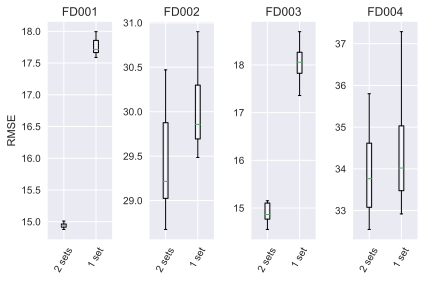
\includegraphics[width=0.5\textwidth]{img/rmse_comparisson.png}
\caption{Comparison of \gls{rmse} results for different sets of data-related parameters.}
\label{fig:scores_rmse}
\end{figure}

\begin{figure}[!htb]
\centering
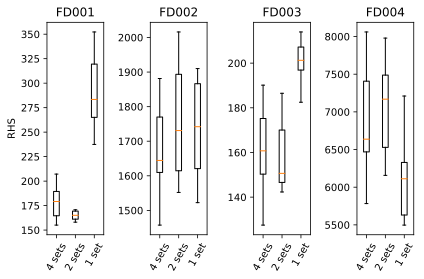
\includegraphics[width=0.5\textwidth]{img/rhs_comparisson.png}
\caption{Comparison of \gls{rhs} results for different sets of data-related parameters.}
\label{fig:scores_rhs}
\end{figure}

\subsection{Comparison with other approaches}

In this section the performance of the proposed method is compared against other state-of-the-art methods. Most of the presented methods in this section have only reported results on the test set FD001 in terms of \gls{rmse}, the results are displayed in Table \ref{table:results_comparison}. The \gls{rmse} value of the proposed method in Table \ref{table:results_comparison} is the mean value of 10 independent runs. The remainder of the values are identical to those reported in their respective original papers.

\begin{table}[!htb]
\centering
\begin{tabular}{l | r r r r | r r r r}
	\hline	
	Method & RMSE \\
  	\hline
  	ESN trained by Kalman Filter \cite{Peng2012} & 63.45\\
  	Support Vector Machine Classifier \cite{Louen2013} & 29.82\\
  	Time Window Neural Network \cite{Lim2016} & 15.16\\
  	Multi-objective deep belief networks ensemble \cite{Zhang2016} & 15.04\\
  	Deep Convolutional Neural Network \cite{Babu2016} & 18.45\\
  	\textbf{Proposed method with $n_w = 30$, $n_s=1$ and $R_e = 128$} & 14.87\\
  	\hline
\end{tabular}
\caption{Performance comparisons of the proposed method and the latest related papers on the \gls{cmaps} dataset.}
\label{table:results_comparison}
\end{table}

Based on the results, the proposed method performs better than the majority of the compared methods when taking into consideration the whole dataset FD001. Two methods come close to the performance of the presented approach in this paper, namely the time window \gls{ann} \cite{Lim2016} and the Networks Ensemble \cite{Zhang2016}. While the performance of both methods comes close to the results presented in this paper, the presented approach is computationally more efficient. Furthermore, the framework proposed in here is simple to understand and implement, robust, generic and light-weight, features we believe are important to highlight when comparing the proposed method against other state-of-the-art approaches.


\section{Conclusions and Future Work}
\label{sec:conclusions}

Here we have presented a novel continuation method for the treatment of \glspl{mmop}. The Enhanced Directed Search (\gls{eds}), as we call our method, follows the ideas proposed by the original Directed Search (\gls{ds}) method \cite{directed_search}. Nevertheless, as indicated by its name, the \gls{eds} method has several improvements over the classical \gls{ds} method. Namely that the \gls{eds} method has a better, more reliable mechanism for determining critical points than the one in the \gls{ds} method (the $\delta$ threshold). Furthermore, the \gls{eds} method is capable of solving \glspl{mmop} through a strategy of rounding which, according the experiments conducted in this work, proved to be efficient and effective. In addition, the performance of the \gls{eds} method can be improved through the use of neighborhood information. 

The experiments conducted here also demonstrated that the \gls{eds} method performs better than its closest competitor, the \gls{dzz} method. A major difference between these two methods is that the former can be used for problems where $k > 2$. This provides clear evidence that the \gls{eds} can be applied to problems that can be solved by the \gls{dzz} and obtain as good results as it and furthermore, that the \gls{eds} method can be applied for solving problems that are impossible to solve for the \gls{dzz} method.

For future work it is intended to test on some other corrector techniques as well as a detailed analysis of convergence of the \gls{eds} method. A version of the \gls{eds} method that does not rely so much on problem dependent parameters is also desirable. The treatment of constrained problems is equally interesting. For the latter task some ideas are being currently explored, nevertheless, they are left out of the scope of this paper. We believe this task to be key for the success of the method in real-world applications.

Another interesting topic that arises from the development of the \gls{eds} method is that of parallelization. Given the way predictors and correctors are computed (Sections \ref{sec:predictor} and \ref{sec:corrector}) and thanks to the successfully implementation of the data structure proposed in \cite{pareto_tracer} we believe that parallelizing the computation of predictors and correctors is an attainable task. A parallel implementation of the \gls{eds} method should boost the speed and the overall performance of it, allowing it to deal in a more efficient way with problems whose function evaluation time is high.

Finally, we would like to stress that the \gls{eds} method (as all continuation methods) is of local nature. It is thus conceivable to hybridize the algorithm with a global strategy such as specialized \glspl{moea} in order to obtain a fast and reliable procedure. Furthermore, the use of neighboring information can be exploited more with the use of memetic strategies where the solutions computed by the \gls{moea} can be reused.

All in all, we strongly believe that the \gls{eds} method has some serious potential for real-world applications, nevertheless, further experiments and some additional features are needed in order to guarantee its success when dealing with real-world problems.
\pagebreak
\appendix
%\addcontentsline{toc}{section}{Appendices}
%\section*{Appendices}
\section{Appendix}
\label{sec:appendices}


Different architectures tested

Architecture 1

\begin{table}[!htb]
\centering
\begin{tabular}{l l l l}
	\hline
	Layer & Shape & Activation & Additional Information\\
  	\hline
  	Fully connected & 30 & ReLU & Dropout(0.6)\\
  	Fully connected & 10 & ReLU & Dropout(0.2)\\
  	Fully connected & 1 & Linear & \\
  	\hline
\end{tabular}
\caption{Proposed Neural Network architecture 1}
\label{table:proposed_nn_1}
\end{table}

Architecture 2

\begin{table}[!htb]
\centering
\begin{tabular}{l l l l}
	\hline
	Layer & Shape & Activation & Additional Information\\
  	\hline
  	Fully connected & 50 & ReLU & Dropout(0.6)\\
  	Fully connected & 20 & ReLU & Dropout(0.2)\\
  	Fully connected & 1 & Linear & \\
  	\hline
\end{tabular}
\caption{Proposed Neural Network architecture 2}
\label{table:proposed_nn_2}
\end{table}

Architecture 3

\begin{table}[!htb]
\centering
\begin{tabular}{l l l l}
	\hline
	Layer & Shape & Activation & Additional Information\\
  	\hline
  	Fully connected & 100 & ReLU & Dropout(0.6)\\
  	Fully connected & 50 & ReLU & Dropout(0.2)\\
  	Fully connected & 1 & Linear & \\
  	\hline
\end{tabular}
\caption{Proposed Neural Network architecture 3}
\label{table:proposed_nn_3}
\end{table}

Architecture 4

\begin{table}[!htb]
\centering
\begin{tabular}{l l l l}
	\hline
	Layer & Shape & Activation & Additional Information\\
  	\hline
  	Fully connected & 250 & ReLU & Dropout(0.6)\\
  	Fully connected & 50 & ReLU & Dropout(0.2)\\
  	Fully connected & 1 & Linear & \\
  	\hline
\end{tabular}
\caption{Proposed Neural Network architecture 4}
\label{table:proposed_nn_4}
\end{table}

\begin{table}[!htb]
\centering
\begin{tabular}{l r r | r r | r r | r r}
	\hline	
	& \multicolumn{2}{c}{Min.} & \multicolumn{2}{c}{Max.}  & \multicolumn{2}{c}{Avg.}  & \multicolumn{2}{c}{STD} \\
	Tested Architecture & RMSE & RHS & RMSE & RHS & RMSE & RHS & RMSE & RHS\\
  	\hline
  	Architecture 1 & 11.09 & 172.18 & 14.98 & 397.79 & 12.96 & 295.51 & 1.27 & 68.62\\
  	Architecture 2 & 11.27 & 187.88 & 14.28 & 344.96 & 12.84 & 274.69 & 0.82 & 42.78\\
  	Architecture 3 & 12.45 & 257.33 & 15.60 & 483.22 & 14.46 & 389.27 & 1.03 & 78.12\\
  	Architecture 4 & 13.26 & 307.14 & 15.58 & 465.33 & 14.57 & 405.08 & 0.74 & 52.03\\
  	\hline
\end{tabular}
\caption{Results for different architectures for subset 1, 250 epochs}
\label{table:tested_architectures_250}
\end{table}

%------------------------------------------------


\vskip 0.2in
\bibliography{../reference_rul_paper}

\end{document}